\documentclass[a4paper,10pt]{scrartcl}
\usepackage[utf8]{inputenc}
\usepackage[T1]{fontenc}
\usepackage{amsmath,amssymb}
\usepackage{lmodern}
\usepackage{pgfplots,tikz}
\usepackage{fullpage}
\usepackage{comment}
\usepackage{siunitx}
\usepackage{biblatex}
\usepackage{physics}

\usetikzlibrary{external,arrows}
\tikzexternalize[prefix=figures/]
\usepgfplotslibrary{colorbrewer}
\usepgfplotslibrary{groupplots}
\pgfplotsset{compat=1.15}
\pgfplotsset{cycle list/Set1}

\bibliography{bibliography}


\newcommand\matder[1]{\frac{D#1}{Dt}}
\newcommand\Gr{\mathrm{Gr}}


% Macro to strech matrices: \begin{pmatrix}[1.5] ... \end{pmatrix}
\makeatletter
\renewcommand*\env@matrix[1][\arraystretch]{%
    \edef\arraystretch{#1}%
    \hskip -\arraycolsep
    \let\@ifnextchar\new@ifnextchar
    \array{*\c@MaxMatrixCols c}}
\makeatother

\subject{LMECA2660 - Numerical Methods in Fluid Mechanics}
\title{Project: Numerical study of the heating of a fluid in a box}
\author{Adrien \textsc{Couplet} \and Marie-Pierre \textsc{van Oldeneel}}

\begin{document}
\maketitle
\section{Introduction}
In this project, it is proposed to study numerically the heating of a fluid in a box and the 2-D flow arising from natural convection. The box has a rectangular shape of sides $L\times H$ and the height is taken as $H=\frac{3}{2}L$. The fluid is initially at a temperature $T_0$. Then, it is heated at the bottom wall with a constant heat flux density $q_w$, while the upper surface, which is opened to the atmosphere at $T_\infty$, undergoes heat losses by forced convection. The convection flux is characterized by an average heat transfer coefficient $\bar{h}$.

The side walls of the box are assumed to be perfectly insulated. Contrary to the side and bottom walls for which a no-slip condition $(u_\Gamma = v_\Gamma=0)$ is applied, the upper surface is a free surface directly in contact with the convective flow above. Hence a no-through flow condition is implemented for this surface:
\begin{equation} \pdv{u}{y} = 0 \qquad\text{and}\qquad v=0 \end{equation}
A statistically stationary state is reached when the heat loss at the free surface balances the heat supply at the bottom of the box. We are interested in the value of the spatially-average temperature,
\begin{equation} \langle T\rangle(t) = \frac{1}{\Omega_f}\int_{\Omega_f}T(\vb{x},t)dS \end{equation}
One of the aims of this project is to determine the time needed to reach a certain average temperature for two modes of operation. First, a configuration where the entire domain is filled with fluid will be studied; the mixing in the box is then solely performed by natural convection. Next a mixer will be introduced in the flow.

The mixer will be taken into account using a penalization method. Inside the body, an extra source term is added to the momentum equation in order to force the flow velocity $\vb{v}$ to match the velocity of the body $\vb{v}_s$. The same strategy is used to impose the temperature of the mixer, $T_s$. At each time step, the temperature of the mixer is assumed to be equal to the spatially averaged fluid temeprature $\langle T\rangle\rvert_{cyl}(t)$ performed on the cylinder of diameter $D$ delimited by the blade's tip of the mixer; i.e. $T_s(t) = \langle T\rangle\rvert_{cyl}(t)$. This approximation is a simplification of the more complex heat transfer phenomena between the mixer and the fluid. The solid domain $\Omega_s$ where these source terms are added is specified using a mask function, $\chi$ defined as
\begin{equation} \chi = \left\{ \begin{aligned} 1 & \text{ for } \vb{x}\in\Omega_s \\ 0 & \text{ elsewhere}\end{aligned}\right. \end{equation}

We will make us of the Boussinesq approximation: the change of density is only taken into account via a buoyancy term in the momentum equation, while the flow is still assumed incompressible. Moreover, the Eckert number will be assumed very small:
\begin{equation} Ec = \frac{U^2}{c_p\Delta T} << 1 \end{equation}
so that the viscous dissipation can be neglected in the energy equation.

The equation to solve are then obtained as:
\begin{align}
        \div\vb{v} &= 0 \label{eq:tosolve1}\\
        \matder{\vb{v}} &= -\grad P + \nu\laplacian\vb{v} - \beta(T-T_0)\vb{g} - \chi\frac{(\vb{v}-\vb{v}_s)}{\Delta \tau} \label{eq:tosolve2}\\
        \matder{T} &= \alpha\laplacian T - \chi\frac{(T-T_s)}{\Delta \tau} \label{eq:tosolve3}
\end{align}
with $\nu = \frac{\mu}{\rho_0}$ the kinematic viscosity, $P=\frac{(p-p_\mathrm{ref})+\rho_0gy}{\rho_0}$ the reduced pressure ($p_\mathrm{ref}$ is any reference pressure), $\vb{g} = -g\hat{e}_y$ the gravitational acceleration, $\beta = -\frac{1}{\rho_0}\pdv{\rho}{T}\rvert_0$ the fluid expansion coefficient and $\Delta\tau$ a parameter to fix, and with dimension of time (the smaller $\Delta\tau$, the better the presence of the mixer into the flow is taken into account).

The fluid Prandtl number is taken as $Pr = \frac{\nu}{\alpha} = 2.0$. We define that the heat flux density at the bottom wall is $q_w = \frac{k\Delta T}{H}$: this defines the reference temperature difference $\Delta T$. We also define the reference velocity $U=\sqrt{\beta g\Delta TH}$. The Grashof number is $Gr = \left(\frac{UH}{\nu}\right)^2 = \num{2.0e10}$. The convective heat transfer at the top surface can also be written as
\begin{equation} \pdv{T}{y} + \frac{1}{l_0}(T-T_\infty) = 0 \end{equation}
where $l_0 = \frac{k}{h}$ has the dimension of a length. We assume that $l_0 = \num{1.0e-3}H$. The temperature of the convective flow above is such that $\frac{T_0-T_\infty}{\Delta T} = \num{5.0e-3}$.

In order to integrate equations (\ref{eq:tosolve1}), (\ref{eq:tosolve2}), (\ref{eq:tosolve3}), we use a two-step projection scheme combined with a MAC mesh. The convective terms are integrated using the Adams-Bashforth scheme of order 2 (with the explicit Euler scheme for the first step) while the diffusive terms are integrated using the explicit Euler scheme. Hence, the numerical scheme is:
\begin{align}
    \frac{(\vb{v}^*-\vb{v}^n)}{\Delta t} &= -\frac{1}{2}(3\vb{H}^n-\vb{H}^{n-1}) - \grad_hP^n + \nu\laplacian_h\vb{v}^n - \beta(T^n-T_0)\vb{g} - \chi\frac{(\vb{v}^*-\vb{v}_s^{n+1})}{\Delta\tau} \label{eq:flow_solving1}\\
    \laplacian_h\Phi &= \frac{1}{\Delta t}\vb{\nabla}_h\vdot\vb{v}^* \label{eq:poisson}\\
    \frac{(\vb{v}^{n+1}-\vb{v}^*)}{\Delta t} &= -\grad_h\Phi \\
    P^{n+1} &= P^n + \Phi \\
    \frac{(T^{n+1}-T^n)}{\Delta t} &= -\frac{1}{2}(3H^n_T - H^{n-1}_T) + \alpha\laplacian_hT^n - \chi\frac{(T^{n+1}-T_s^{n+1})}{\Delta\tau}
\end{align}
where $\vb{H}$ is the convective term of the momentum equation and $H_T$ is the convective term of the energy equation.

The Poisson equation (\ref{eq:poisson}) is solved using the over-relaxed Gauss-Seidel algorithm (SOR):
\begin{align} 
    \Phi_{i,j}^* &= \frac{1}{2}\frac{(\Delta x)^2(\Delta y)^2}{\left((\Delta x)^2 + (\Delta y)^2\right)}\left(-\frac{1}{\Delta t}(\vb{\nabla}_h\vdot\vb{v}^*)_{i,j} + \frac{(\Phi^k_{i+1,j} + \Phi^{k+1}_{i-1,j})}{(\Delta x)^2} + \frac{(\Phi^k_{i,j+1} + \Phi^{k+1}_{i,j-1})}{(\Delta y)^2}\right), \\
    \Phi^{k+1}_{i,j} &= \alpha\Phi^*_{i,j} + (1-\alpha)\Phi^k_{i,j},
\end{align}
with $1 \leq \alpha < 2$ the relaxation parameter ($\alpha = 1.97 - 1.98$ should provide an optimal convergence rate). The local residual of the Poisson equation is defined as:
\begin{equation} R^{k+1}_{i,j} = (\laplacian_h\Phi)_{i,j} - \frac{1}{\Delta t}(\vb{\nabla}_h\vdot\vb{v}^*)_{i,j}. \end{equation}
The global error on the solution of the Poisson equation is defined as:
\begin{equation} e^{k+1} = \Delta t\frac{H}{U}\sqrt{\frac{1}{LH}\sum_i^{n_x}\sum_j^{n_y}(R_{i,j}^{k+1})^2\Delta x \Delta y}, \end{equation}
This diagnostic must be evaluated at every time step in order to ensure the convergence of the iterative process.

We will here use a mesh with $\Delta x = \Delta y = h$, where $h$ fulfills a constraint on the precision of the solution, that is to say that $Re_h = \frac{(|u|+|v|)h}{\nu}$ must be ``sufficiently moderate''. The time step $\Delta t$ is chosen so that the stability of the problem is ensured (in which the factors $r = \frac{\nu\Delta t}{h^2}$ and $CFL = \frac{(|u|+|v|)\Delta t}{h} = rRe_h$ are involved). The parameter $\Delta\tau$ is chosen relatively to the time step: $\frac{\Delta t}{\Delta\tau}$ is taken as a large number (e.g., \num{1.0e3}).

For flows with large local gradients of the computed quantities, a more appropriate definite of the ``mesh Reynolds number'' is that based on the vorticity: $Re_{h,\omega} = \frac{|\omega|h^2}{\nu}$. Acceptable values for quality simulations are $Re_{h,\omega} \leq 40$, and $Re_h \leq 25$. Hence, we will monitor the maximum value of $Re_h$ and $Re_{h,\omega}$ of our simulations as a function of time.

Two cases will be considered:
\begin{enumerate}
    \item In a first step, the entire domain is filled with fluid ($\Omega = \Omega_f$); thus the mixing in the box is solely performed by natural convection.
    \item In a second step, a mixer is introduced, with its center located at $x_g = y_g = \frac{L}{2}$. The solid domain $\Omega_s$ consists of the superposition of a three-petals rose of diameter $D = 2a = \frac{3}{5}L$ and of equation $r=a\cos(3\theta)$, and of a disk of diameter $d=\frac{D}{5}$. The angular velocity of the mixer is set to $\frac{\omega_sH}{U} = \num{1.0e-1}$.
\end{enumerate}

\section{Numerical code}
\subsection{The MAC grid \label{sec:MACgrid}}
The problem is solved on a staggered ``marker and cell'' (MAC) mesh (first described in \cite{harlow1965numerical}). A two-dimensional MAC grid cell (Figure~\ref{fig:MACgrid}) defines the $x$ component of a cell's velocity on the vertical faces and the $y$ component on the horizontal faces. Pressure and temperature are defined at the center of the MAC cells. We use a half index notation, so for cell $(i,j)$ in two dimensions we have $P_{i,j}$ and $T_{i,j}$ at the center, and $u_{i-\frac{1}{2},j}$, $u_{i+\frac{1}{2},j}$, $v_{i,j-\frac{1}{2}}$ and $v_{i,j+\frac{1}{2}}$ normal to the faces. MAC meshes are also well suited for solid wall boundaries and free surface boundaries. Solid wall boundaries involve setting the normal velocity on a boundary to zero or $\vb{v}\vdot\hat{n} = 0$. This is trivial for grid aligned solids on a MAC grid since velocities are stored perpendicular to cell faces.
\begin{figure}[ht]\centering
    \tikzsetnextfilename{MACgrid} 
    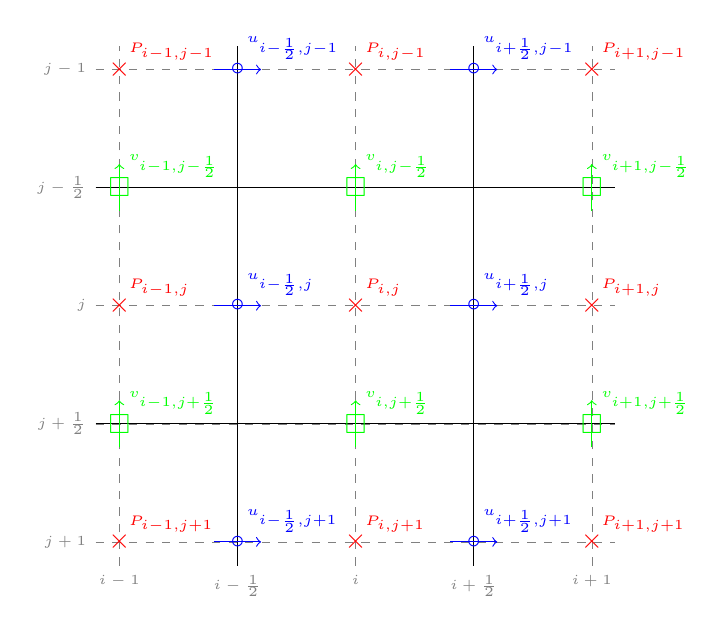
\begin{tikzpicture}[font=\tiny]
        \foreach \i in {0,...,4}{
            \draw[very thin,gray,dashed] (1.5*\i,-0.3) -- (1.5*\i,6.3);
            \draw[very thin,gray,dashed] (-0.3,1.5*\i) -- (6.3,1.5*\i);
        }
        \foreach \i in {0,...,2}{
            \foreach \j in {0,...,2}{
                \node[red] at (\i*3,\j*3) {\normalsize$\times$};
            }
        }
        \foreach \i in {0,...,1}{
            \draw[black] (3*\i+1.5,-0.3) -- (3*\i+1.5,6.3);
            \draw[black] (-0.3,3*\i+1.5) -- (6.3,3*\i+1.5);
            \foreach \j in {0,...,2}{
                \node[blue] at (\i*3+1.5,\j*3) {\normalsize$\circ$};
                \draw[blue,->] (\i*3+1.5-0.3,\j*3) -- (\i*3+1.5+0.3,\j*3);
                \node[green] at (\j*3,\i*3+1.5) {\normalsize$\square$};
                \draw[green,->] (\j*3,\i*3++1.5-0.3) -- (\j*3,\i*3+1.5+0.3);
            }
        }

        \node[left,gray] at (-0.3,0) {$j+1$};
        \node[left,gray] at (-0.3,1.5) {$j+\frac{1}{2}$};
        \node[left,gray] at (-0.3,3) {$j$};
        \node[left,gray] at (-0.3,4.5) {$j-\frac{1}{2}$};
        \node[left,gray] at (-0.3,6) {$j-1$};
        \node[below,gray] at (0,-0.3) {$i-1$};
        \node[below,gray] at (1.5,-0.3) {$i-\frac{1}{2}$};
        \node[below,gray] at (3,-0.3) {$i$};
        \node[below,gray] at (4.5,-0.3) {$i+\frac{1}{2}$};
        \node[below,gray] at (6,-0.3) {$i+1$};
        \node[above right,red] at (0,0) {$P_{i-1,j+1}$};
        \node[above right,red] at (3,0) {$P_{i,j+1}$};
        \node[above right,red] at (6,0) {$P_{i+1,j+1}$};
        \node[above right,red] at (0,3) {$P_{i-1,j}$};
        \node[above right,red] at (3,3) {$P_{i,j}$};
        \node[above right,red] at (6,3) {$P_{i+1,j}$};
        \node[above right,red] at (0,6) {$P_{i-1,j-1}$};
        \node[above right,red] at (3,6) {$P_{i,j-1}$};
        \node[above right,red] at (6,6) {$P_{i+1,j-1}$};
        \node[above right,blue] at (1.5,0) {$u_{i-\frac{1}{2},j+1}$};
        \node[above right,blue] at (4.5,0) {$u_{i+\frac{1}{2},j+1}$};
        \node[above right,blue] at (1.5,3) {$u_{i-\frac{1}{2},j}$};
        \node[above right,blue] at (4.5,3) {$u_{i+\frac{1}{2},j}$};
        \node[above right,blue] at (1.5,6) {$u_{i-\frac{1}{2},j-1}$};
        \node[above right,blue] at (4.5,6) {$u_{i+\frac{1}{2},j-1}$};
        \node[above right,green] at (0,1.5) {$v_{i-1,j+\frac{1}{2}}$};
        \node[above right,green] at (0,4.5) {$v_{i-1,j-\frac{1}{2}}$};
        \node[above right,green] at (3,1.5) {$v_{i,j+\frac{1}{2}}$};
        \node[above right,green] at (3,4.5) {$v_{i,j-\frac{1}{2}}$};
        \node[above right,green] at (6,1.5) {$v_{i+1,j+\frac{1}{2}}$};
        \node[above right,green] at (6,4.5) {$v_{i+1,j-\frac{1}{2}}$};

    \end{tikzpicture}
    \caption{Staggered ``marker and cell'' (MAC) mesh}
    \label{fig:MACgrid}
\end{figure}
\subsection{The equations}
We now rewrite the equations needed to solve the problem in order to easily put them in our code. We have to take into account the particularities of the MAC grid and the used integration schemes. For the convective terms we use the Adams-Bashforth scheme of order 2 (with the explicit Euler scheme for the first step) while the diffusive terms are integrated using the explicit Euler scheme.
\paragraph{Equation (\ref{eq:flow_solving1})}
We start by detailing every term of equation (\ref{eq:flow_solving1}):
\begin{equation} \underbrace{\frac{(\vb{v}^*-\vb{v}^n)}{\Delta t}}_{(1)} = \underbrace{-\frac{1}{2}(3\vb{H}^n-\vb{H}^{n-1})}_{(2)} - \underbrace{\grad_nP^n}_{(3)} + \underbrace{\nu\laplacian_n\vb{v}^n}_{(4)} - \underbrace{\beta(T^n-T_0)\vb{g}}_{(5)} - \underbrace{\chi\frac{(\vb{v}^*-\vb{v}_s^{n+1})}{\Delta\tau}}_{(6)} \label{eq:ns1}\end{equation}

Term (\ref{eq:ns1}.1) corresponds to the time-dependent component of the inertial term. We can rewrite it as
\begin{equation} \frac{1}{\Delta t}\begin{pmatrix} u^*_{i+\frac{1}{2},j} - u^n_{i+\frac{1}{2},j} \\ v^*_{i,j+\frac{1}{2}} - v^n_{i,j+\frac{1}{2}} \end{pmatrix} \end{equation}

Term (\ref{eq:ns1}.2) corresponds to the Adams-Bashforth scheme of order 2 of the convective component of the inertial term. First we need to write out $\vb{H}$.  This term can take both the advective form ($(\vb{\nabla}\vb{v})\vdot\vb{v}$) and the divergence form ($\vb{\nabla}\vdot(\vb{v}\vb{v})$). The skew-symmetric form is the combination of these two previous forms. This form conserves the kinetic eneryg when $\nu=0$ and conserves the momentum when the continuity is satisfied. We first take a look at the advective form of Kajishima, written as
\begin{align} 
    H_x(\mathrm{Adv.}) &= u\pdv{u}{x} + v\pdv{u}{y} \\
        &= \overline{\overline{u}^x\fdv{u}{x}}^x + \overline{\overline{v}^x\fdv{u}{y}}^y \\
\end{align}
where the mean value in the direction $x$ and $y$ are expressed as
\begin{align}
    \overline{u}^x_{i,j} &\triangleq \frac{1}{2}\left(u_{i+\frac{1}{2},j} + u_{i-\frac{1}{2},j}\right) \\
    \overline{v}^y_{i,j} &\triangleq \frac{1}{2}\left(v_{i,j+\frac{1}{2}} + v_{i,j-\frac{1}{2}}\right) \\
    \overline{u}^y_{u+\frac{1}{2},j+\frac{1}{2}} &\triangleq \frac{1}{2}\left(u_{i+\frac{1}{2},j+1} + u_{i+\frac{1}{2},j}\right) \\
    \overline{v}^x_{i+\frac{1}{2},j+\frac{1}{2}} &\triangleq \frac{1}{2}\left(v_{i+1,j+\frac{1}{2}} + v_{i,j+\frac{1}{2}}\right) 
\end{align}
We now can write the complete advective form of Kajishima
\begin{align}
    H_{x,i+\frac{1}{2},j} &= \frac{1}{2}\left(\left(\overline{u}^x\fdv{u}{x}\right)_{i+1,j} + \left(\overline{u}^x\fdv{u}{x}\right)_{i,j}\right) + \frac{1}{2}\left(\left(\overline{v}^x\fdv{u}{y}\right)_{i+\frac{1}{2},j+\frac{1}{2}} + \left(\overline{v}^x\fdv{u}{y}\right)_{i+\frac{1}{2},j-\frac{1}{2}}\right) \\
        &= \frac{1}{2}\left(\frac{(u_{i+\frac{3}{2},j} + u_{i+\frac{1}{2},j})(u_{i+\frac{3}{2},j}-u_{i+\frac{1}{2},j})}{2\Delta x} + \frac{(u_{i+\frac{1}{2},j} + u_{i-\frac{1}{2},j})(u_{i+\frac{1}{2},j}-u_{i-\frac{1}{2},j})}{2\Delta x}\right) \nonumber\\
        &+ \frac{1}{2}\left(\frac{(v_{i+1,j+\frac{1}{2}} + v_{i,j+\frac{1}{2}})(u_{i+\frac{1}{2},j+1} - u_{i+\frac{1}{2},j})}{2\Delta y} + \frac{(v_{i+1,j-\frac{1}{2}} + v_{i,j-\frac{1}{2}})(u_{i+\frac{1}{2},j} - u_{i+\frac{1}{2},j-1})}{2\Delta y}\right)
\end{align}
Secondly, we take a look at the divergence form 
\begin{align}
	H_x(\mathrm{Div.}) &= \frac{\partial}{\partial x}(uu) + \frac{\partial}{\partial y}(vu) \\
		&= \frac{\delta}{\delta x}(\overline{u}^x\overline{u}^x) + \frac{\delta}{\delta y}(\overline{v}^x\overline{u}^y)
\end{align}
The complete divergence form is now
\begin{align}
	H_{x,i+\frac{1}{2},j} &= \frac{1}{\Delta x}\left(\overline{u}^x_{i+1,j}\overline{u}^x_{i+1,j} - \overline{u}^x_{i,j}\overline{u}^x_{i,j}\right) + \frac{1}{\Delta y}\left(\overline{v}^x_{i+\frac{1}{2},j+\frac{1}{2}}\overline{u}^y_{i+\frac{1}{2},j+\frac{1}{2}} - \overline{v}^x_{i+\frac{1}{2},j-\frac{1}{2}}\overline{u}^y_{i+\frac{1}{2},j-\frac{1}{2}}\right) \\
		&= \frac{(u_{i+\frac{3}{2},j}+u_{i+\frac{1}{2},j})^2-(u_{i+\frac{1}{2},j}+u_{i-\frac{1}{2},j})^2}{4\Delta x} \nonumber\\
		&+ \frac{(v_{i+1,j+\frac{1}{2}}+v_{i,j+\frac{1}{2}})(u_{i+\frac{1}{2},j+1}+u_{i+\frac{1}{2},j})-(v_{i+1,j-\frac{1}{2}}+v_{i,j-\frac{1}{2}})(u_{i+\frac{1}{2},j}+u_{i+\frac{1}{2},j-1})}{4\Delta y}
\end{align}	
Finally we obtain the convective component of the inertial term in the skew-symmetric form
\begin{equation}
	H_{x,i+\frac{1}{2},j}(\mathrm{SS.}) = \frac{1}{2}H_{x,i+\frac{1}{2},j}(\mathrm{Adv.}) + \frac{1}{2}H_{x,i+\frac{1}{2},j}(\mathrm{Div.})
\end{equation}
The component of $\vb{H}$ in the $y$-direction is obtained as follow
\begin{align}
	H_{y,i,j+\frac{1}{2}}(\mathrm{SS.}) &= \frac{1}{2}H_{y,i,j+\frac{1}{2}}(\mathrm{Adv.}) + \frac{1}{2}H_{y,i,j+\frac{1}{2}}(\mathrm{Div.}) \\
		&= \frac{1}{2}\left(\overline{\overline{u}^y\fdv{v}{x}}^x + \overline{\overline{v}^y\fdv{v}{y}}^y\right)_{i,j+\frac{1}{2}} + \frac{1}{2}\left(\frac{\delta}{\delta x}(\overline{u}^y\overline{v}^x) + \frac{\delta}{\delta y}(\overline{v}^y\overline{v}^y)\right)_{i,j+\frac{1}{2}}
\end{align}
The final form of Term (\ref{eq:ns1}.2) is
\begin{equation} \begin{pmatrix}H_{x,i+\frac{1}{2},j}(\mathrm{SS.}) \\ H_{y,i,j+\frac{1}{2}}(\mathrm{SS.})\end{pmatrix} \end{equation}

Term (\ref{eq:ns1}.3) corresponds to the pressure term of the Navier-Stokes equation. The complete expression of this term is
\begin{equation} \begin{pmatrix} \pdv{P}{x}\rvert_{i+\frac{1}{2},j} \\ \pdv{P}{y}\rvert_{i,j+\frac{1}{2}} \end{pmatrix}  = \begin{pmatrix} \frac{P_{i+1,j}-P_{i,j}}{\Delta x} \\ \frac{P_{i,j+1} - P_{i,j}}{\Delta y} \end{pmatrix}\end{equation}

Term (\ref{eq:ns1}.4) corresponds to the diffusion term of the Navier-Stokes equation. We integrate it using the explicit Euler scheme
\begin{equation} \nu\begin{pmatrix} \left(\pdv[2]{u}{x} + \pdv[2]{u}{y}\right)\rvert_{i+\frac{1}{2},j} \\ \left(\pdv[2]{v}{x} + \pdv[2]{v}{y}\right)\rvert_{i,j+\frac{1}{2}} \end{pmatrix} = \nu\begin{pmatrix} \frac{u_{i+\frac{3}{2},j}-2u_{i+\frac{1}{2},j}+u_{i-\frac{1}{2},j}}{(\Delta x)^2} + \frac{u_{i+\frac{1}{2},j+1}-2u_{i+\frac{1}{2},j}+u_{i+\frac{1}{2},j-1}}{(\Delta y)^2} \\ \frac{v_{i+1,j+\frac{1}{2}}-2v_{i,j+\frac{1}{2}}+v_{i-1,j+\frac{1}{2}}}{(\Delta x)^2} + \frac{v_{i,j+\frac{3}{2}}-2v_{i,j+\frac{1}{2}}+v_{i,j-\frac{1}{2}}}{(\Delta y)^2} \end{pmatrix}\end{equation}

Term (\ref{eq:ns1}.5) corresponds to buoyancy term needed to take into account the change of density. It is expressed as 
\begin{equation} -\beta\begin{pmatrix} (T-T_0)\vdot 0\rvert_{i+\frac{1}{2},j} \\ (T-T_0)\vdot g\rvert_{i,j+\frac{1}{2}} \end{pmatrix}  = -\beta\begin{pmatrix} 0 \\ \left(\frac{T_{i,j+1}+T_{i,j}}{2} - T_0\right)g \end{pmatrix}\end{equation} 

Term (\ref{eq:ns1}.6) corresponds to an extra source term used to take into account the mixer using a penalization method. It is expressed as
\begin{equation} \frac{\chi}{\Delta\tau}\begin{pmatrix} u^*_{i+\frac{1}{2},j} - u^{n+1}_{s,i+\frac{1}{2},j} \\ v^*_{i,j+\frac{1}{2}} - v^{n+1}_{s,i,j+\frac{1}{2}} \end{pmatrix} \end{equation}

Using the following dimensionless variables
\begin{align}
	t' &= \frac{tU}{H} & \vb{v'} &= \frac{\vb{v}}{U} & T' &= \frac{T-T_0}{\Delta T} \nonumber\\
	P' &= \frac{P}{U^2} & h' &= \frac{h}{H} & \tau' &= \frac{\tau U}{H} \nonumber
\end{align}
expressing every term in equation (\ref{eq:ns1}) with their fully developed form and replacing the variables $(t,\vb{v},T,P,h,\tau)$ by their dimensionless version would give us
\begin{equation}
	\frac{U^2}{H}(\ref{eq:ns1}.1) = \frac{U^2}{H}(\ref{eq:ns1}.2) + \frac{U^2}{H}(\ref{eq:ns1}.3) + \frac{\nu U}{H^2}(\ref{eq:ns1}.4) + \beta g \Delta T(\ref{eq:ns1}.5) + \frac{U^2}{H}(\ref{eq:ns1}.6)
\end{equation}
where the constant coefficients in front of every term can be expressed by the Grashof number
\begin{equation} \frac{1}{\sqrt{\Gr}}(\ref{eq:ns1}.1) = \frac{1}{\sqrt{\Gr}}(\ref{eq:ns1}.2) + \frac{1}{\sqrt{\Gr}}(\ref{eq:ns1}.3) + \frac{1}{\Gr}(\ref{eq:ns1}.4) + \frac{1}{\sqrt{\Gr}}(\ref{eq:ns1}.5) + \frac{1}{\sqrt{\Gr}}(\ref{eq:ns1}.6) \end{equation}

\section{First case: without mixer}
\section{Second case: with a mixer}
\section{Conclusion}
\section{References}
\printbibliography


\end{document}

